\subsection{Directional diffusion}

Regular diffusion will present noticeable artifacts. These typically occur at high-contrast edges of the image. Because the diffusion kernel equally weighs pixels from all directions it creates a blur effect and is unable to properly propogate edges into the unknown regions. This effect can be seen in figure \ref{fig:stepbystepcross}. To help resolve this problem we use directional kernels that weigh pixels from certain directions more heavily. We define directionality to be the angle in which the high-contrast edges of an image are directed. An image with mostly horizontal lines will have a directionality of $0$ degrees whereas an image with mostly vertical lines will have a directionality of $90$ degrees. By inferring the correct directionality, the artifacts can be noticeably reduced as seen in figure \ref{fig:stepbystepdir}.

To do this we first apply the regular diffusion algorithm to the image to get an estimate of the original image. Then we divide the image into separate patches. For each patch we infer the general directionality by using a heuristic. Based on this directionality we construct a directional kernel. Finally we apply this kernel to do the inpainting for that specific patch. We will now explain these steps in more detail.

\begin{figure*}
	\centering
	\begin{subfigure}[b]{0.3\textwidth}
		\centering
		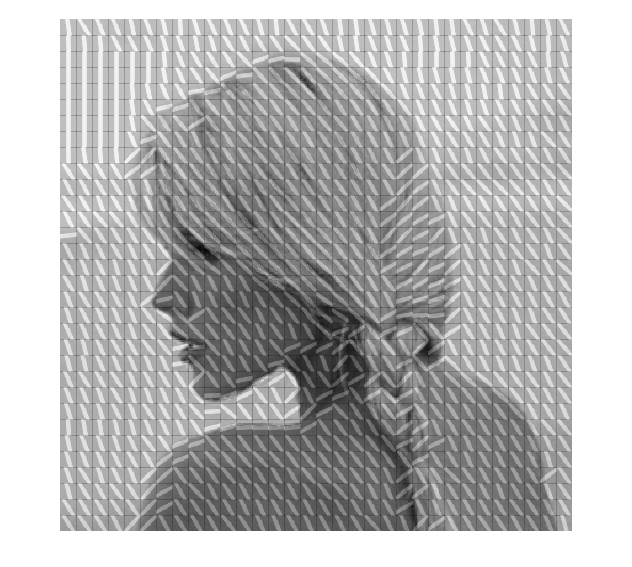
\includegraphics[clip, trim=2cm 0cm 2cm 0cm, width=0.9\textwidth]{figures/claudia-32x32}
		\caption{The claudia image.}
		\label{fig:claudia}
	\end{subfigure}
	\begin{subfigure}[b]{0.3\textwidth}
		\centering
		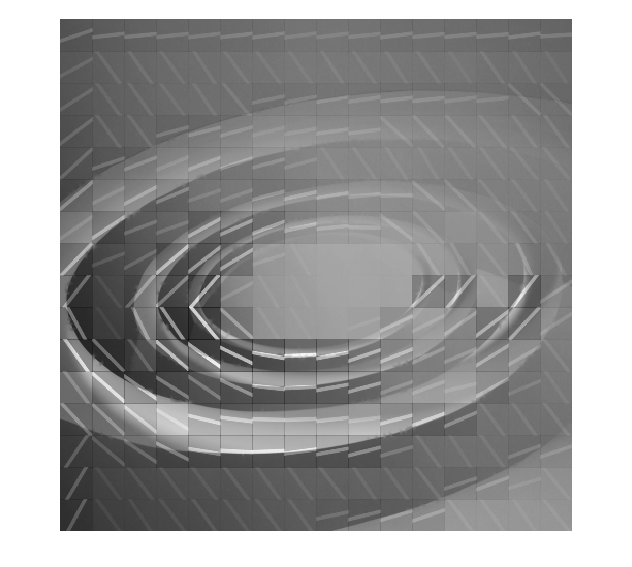
\includegraphics[clip, trim=2cm 0cm 2cm 0cm, width=0.9\textwidth]{figures/spiral-32x32}
		\caption{The spiral image.}
		\label{fig:spiral}
	\end{subfigure}
	\begin{subfigure}[b]{0.3\textwidth}
		\centering
		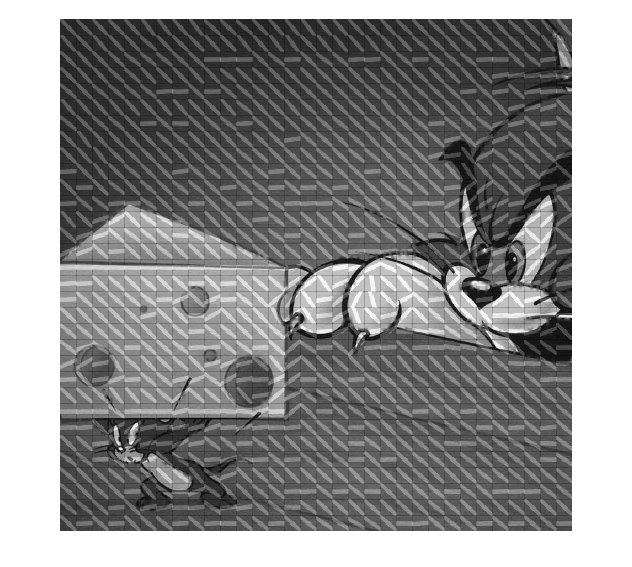
\includegraphics[clip, trim=2cm 0cm 2cm 0cm, width=0.9\textwidth]{figures/tomandjerry-32x32}
		\caption{The tom and jerry image.}
		\label{fig:spiral}
	\end{subfigure}
	
	\caption{The directionality of 16x16 pixel patches shown as white lines.}
	\label{fig:directionality}
\end{figure*}

\subsubsection{Divide image into $n \times n$ patches}
The directionality of the contents of an image is typically a local property. Hence we want to know what the directionality of a small image patch is. An image $I$ can be broken down into patches of size $n \times n$. We define a patch $P$ starting at pixel location $i,j$ as:
\begin{flalign*}
P = \begin{bmatrix}
I_{i,j} & I_{i+1, j} & \hdots & I_{i+n, j}\\
I_{i,j+1} & I_{i+1, j+1} & \hdots & I_{i+n, j+1}\\
\vdots & \vdots & \ddots & \vdots \\
I_{i, j+n} & I_{i+1, j+n} & \hdots & I_{i+n, j+n}
\end{bmatrix}
\end{flalign*}

\subsubsection{Infer directionality of an image patch}
Given an image patch $P$ we wish to compute an estimated angle $\theta$ of the contents of this patch. Intuitively this means for patches with lots of horizontal stripes we would get $\theta \approx 0\degree$ and for patches with lots of vertical stripes we would get $\theta \approx 90\degree$. The first thing we need is a shift operator for matrices. Given a matrix $M \in \mathbb{R}^{n\times m}$ we can compute the shifted matrix $M^{(x,y)}$, which circularly shifts columns towards the right $x$ times and rows towards the bottom $y$ times:
\begin{flalign*}
M^{(x, y)}_{i, j} &= M_{(i + x) \text{ mod } n, (j + y)\text{ mod } m}
\end{flalign*}
Using this shift operator, we compute two basic metrics on the image patch:
\begin{flalign*}
v &= \sum_{i, j}  | P_{i,j} - P_{i,j}^{(1, 0)} | \\
h &= \sum_{i, j} | P_{i,j} - P_{i,j}^{(0, 1)} | 
\end{flalign*}
The first metric $v$ checks how much each pixel differs from the one left of it and provides large values for images with a lot of vertical stripes. The second metric $h$ does the same but checks how much each pixel differs from the one below it. This gives large values for images with a lot of horizontal stripes.

By comparing $h$ and $v$ we can determine if the contents of the image patch will have mostly vertical lines ($v > h$), mostly horizontal lines ($v < h$) or diagonal lines ($v \approx h$). We can turn this into an angle, by computing the fraction of $h$ to $h + v$.  We add $1$ to both sides to prevent division by zero:
\begin{flalign*}
\theta_1 &= 90 \frac{h + 1}{h + v + 1}
\end{flalign*}

A problem with this approach is that it only gives an angle from 0$\degree$ to 90$\degree$. It cannot infer if the diagonal lines on the image patch are left-slanted or right-slanted since these will have $h \approx v$. To help resolve this we propose a heuristic for the diagonal slant by computing $d$, which checks how much each pixel differs from the one diagonally right-below it. This gives large values for images with right-slanted diagonal lines but small values for images with left-slanted diagonal lines. We wish to normalize this value by dividing it by $v+h$, so it ranges from 0 to 1. We add 1 to both sides to prevent division by zero:
\begin{flalign*}
d &= \frac{1 + \sum_{i, j} | P_{i,j} - P_{i,j}^{(1, 1)} |}{1 + v + h}
\end{flalign*}

If this value $d$ is close to 1, we can assume the image is right-slanted. If it is close to 0, we can assume the image is left-slanted. A value close to 0.5 indicates that the image patch has both left and right slanted lines. We can now compute the angle $\theta$ with the additional parameter $d$ using the following heuristic:
\begin{flalign*}
\theta &=  - 90 + \begin{cases}
90d+\theta_1 & \text{if } d > 0.6 \\
90-\theta_1       & \text{if } d \leq 0.6
\end{cases}
\end{flalign*}

In figure \ref{fig:directionality} we show the angle $\theta$, which has been computed on image patches of size $32 \times 32$, as white lines. The heuristic works well on image patches where the contents is simple and consists of mostly straight lines. When the contents of an image patch gets more complex, inferring the angle becomes more difficult and the heuristic fails.

\subsubsection{Constructing a directional kernel}
After computing the angle $\theta$ for an image patch, we wish to construct a directional kernel $K_\theta$, which puts more weight on pixels that align with the angle $\theta$. We start with a diagonal kernel $K_{\text{diag}}$ (see figure \ref{fig:kernels}). This kernel is converted to a $3\times 3$ image which is rotated by $\theta+45$ degrees (because the initial kernel was diagonal, we add 45 degrees) and cropped to obtain a new $3\times 3$ image representing the rotated kernel. During the rotation process, bicubic interpolation is used to smooth the intermediate values. The resulting image is converted back to a $3 \times 3$ matrix representing the kernel $K_\theta$.

\subsubsection{Per-patch diffusion using $K_\theta$}
Now that we have a kernel $K_\theta$ for each image patch $P$ we can run the diffusion algorithm (see algorithm \ref{alg:diffusion}) on each of the patches. The reconstructed image is created by putting all the patches back together after running the diffusion algorithm on them.

